%\renewcommand{\theequation}{\theenumi}
%\begin{enumerate}[label=\arabic*.,ref=\thesubsection.\theenumi]
%\numberwithin{equation}{enumi}
%
\item The vertices of $\triangle ABC$ are $\vec{A}=\myvec{4\\6},  \vec{B}=\myvec{1\\5}$ and  $\vec{C} =  \myvec{7\\2}$.  A line is drawn to intersect sides $AB$ and $AC$ at $D$ and $E$ respectively, such that
\begin{align}
\frac{AD}{AB}=\frac{AE}{AC}= \frac{1}{4}
\end{align}
%
Find 
\begin{align}
\frac{\text{area of }\triangle ADE}{\text{area of }\triangle ABC}.
\end{align}
\item Let $\vec{A}=\myvec{4\\2},  \vec{B}=\myvec{6\\5}$ and  $\vec{C} =  \myvec{1\\4}$ be the vertices of $\triangle ABC$.
\begin{enumerate}
\item The median from $\vec{A}$ meets $BC$ at $\vec{D}$.  Find the coordinates of the point $\vec{D}$.
\item Find the coordinates of the point $\vec{P}$ on $AD$ such that $AP:PD = 2:1$.
\item Find the coordinates of the points $\vec{Q}$ and $\vec{R}$ on medians $BE$ and $CF$ respectively such that $BQ:QE = 2:1$ and $CR:RF = 2:1$.
\end{enumerate}
\solution



\begin{figure}[!ht]
    \centering
    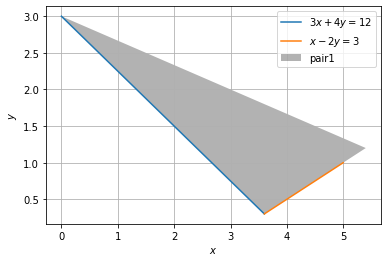
\includegraphics[width=\columnwidth]{solutions/su2021/2/56/Figure9_1.png}
    \caption{Inequality pair 1}
    \label{ineq/56/fig:inequalities1}	
    \end{figure}
    
    \begin{figure}[!ht]
    \centering
    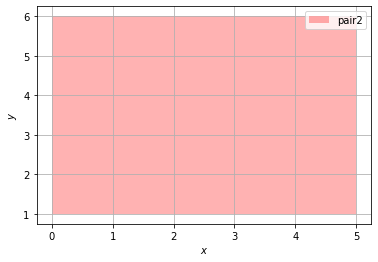
\includegraphics[width=\columnwidth]{solutions/su2021/2/56/Figure9_2.png}
    \caption{Inequality pair 2}
    \label{ineq/56/fig:inequalities2}	
    \end{figure}
    
    \begin{figure}[!ht]
    \centering
    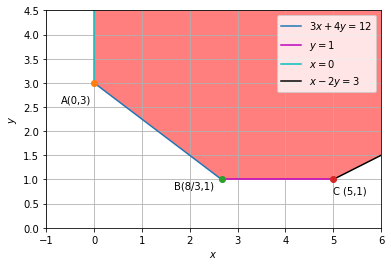
\includegraphics[width=\columnwidth]{solutions/su2021/2/56/Figure 9_3.png}
    \caption{Intersection of \ref{ineq/56/fig:inequalities1} and \ref{ineq/56/fig:inequalities2}}
    \label{ineq/56/fig:inequality3}	
    \end{figure}
    The common region shown by \ref{ineq/56/fig:inequality3} is the solution of set of inequalities.
    
\item In $\triangle ABC$, Show that the centroid 
\begin{align}
\vec{O} = \frac{\vec{A}+\vec{B}+\vec{C}}{3}
\end{align}
\item Show that the points 
\begin{align}
\vec{A} = \myvec{2\\-1 \\1},
\vec{B} = \myvec{1\\-3 \\-5},
\vec{C} = \myvec{3\\ -4\\-4}
\end{align}
%
are the vertices of a right angled triangle.
\item In $\triangle ABC$, 
$
\vec{A} = \myvec{1\\2 \\3},
\vec{B} = \myvec{-1\\0 \\0},
\vec{C} = \myvec{0\\ 1\\2}.
$
Find $\angle B$.
\item Show that the vectors 
$
\myvec{2\\-1 \\1},
\myvec{1\\-3 \\-5},
\myvec{3\\ -4\\-4}
$
form the vertices of a right angled triangle.
\item Find the area of a triangle having the points 
$
\vec{A} = \myvec{1\\1 \\1},
\vec{B} = \myvec{1\\2 \\3}, \text{ and }
\vec{C} = \myvec{2\\ 3\\1}
$
as its vertices.
\item Find the area of a triangle with vertices
$
\vec{A} = \myvec{1\\1 \\2},
\vec{B} = \myvec{2\\3 \\5}, \text{ and }
\vec{C} = \myvec{1\\ 5\\5}
$
\item Find the direction vectors of the sides of a triangle with vertices
$
\vec{A} = \myvec{3\\5 \\-4},
\vec{B} = \myvec{-1\\1 \\2}, \text{ and }
\vec{C} = \myvec{-5\\ -5\\-2}
$
\item Check whether 
\begin{align}
\myvec{5\\-2}, \myvec{6\\4}, \myvec{7\\-2}
\end{align}
are the vertices of an isosceles triangle.
%
 \item Are the points 
\begin{align}
\vec{A} = \myvec{3\\6 \\9},
\vec{B} = \myvec{10\\20 \\30},
\vec{C} = \myvec{25\\ -41\\5},
\end{align}
%
the vertices of a right angled triangle?
\item Determine if the points 
\begin{align}
\myvec{1\\5}, \myvec{2\\3}, \myvec{-2\\-11}
\end{align}
%
are collinear.	
\item By using the concept of equation of a line, prove that the three points \myvec{3\\ 0}, \myvec{– 2\\ – 2} and \myvec{8\\ 2} are collinear.
\item Find the value of $x$ for which the points $\myvec{x\\ – 1}$, \myvec{2\\1} and \myvec{4\\ 5} are collinear.
\item  In each of the following, find the value of $k$ for which the points are collinear

\begin{enumerate}
\item \myvec{7\\-2},  \myvec{5\\1},  \myvec{3\\k} 
\item \myvec{8\\1},  \myvec{k\\-4},  \myvec{2\\-5} 
\end{enumerate}
\item Find a condition on $\vec{x}$  such that the points $\vec{x}, \myvec{1\\2}\myvec{7\\0}$ are collinear.
\item Show that the points 
$\vec{A}=\myvec{1\\2\\7}, \vec{B}=\myvec{2\\6\\3}$ and $ \vec{C}=\myvec{3\\10\\-1}$ are collinear.
\item Show that the points 
$\vec{A}=\myvec{1\\-2\\8}, \vec{B}=\myvec{5\\0\\-2}$ and $ \vec{C}=\myvec{11\\3\\7}$ are collinear, and find the ratio in which $\vec{B}$ divides $AC$.
\item Show that 
$
\vec{A}=\myvec{2\\3\\4}, 
\vec{B}=\myvec{-1\\-2\\1} \text{ and } 
\vec{C}=\myvec{5\\8\\7}$  
are collinear.

\item A bullet fired at an angle of 30$\degree$ with the horizontal hits the ground 3.0 km away. By adjusting its angle of projection, can one hope to hit a target 5.0 km away ? Assume the muzzle speed to be fixed, and neglect air resistance.
\item  A fighter plane flying horizontally at an altitude of 1.5 km with speed 720 km/h passes directly overhead an anti-aircraft gun. At what angle from the vertical should the gun be fired for the shell with muzzle speed 600 $m s^{-1}$ to hit the plane ? 
At what minimum  altitude should the pilot fly the plane to avoid being hit ? (Take g = 10$ m s^{-2}$
).
\item Give the magnitude and direction of the net force acting on a stone of mass 0.1 kg, 
\begin{enumerate}
\item  just after it is dropped from the window of a stationary train, 
\item  just after it is dropped from the window of a train running at a constant velocity of 36 km/h,
\item  just after it is dropped from the window of a train accelerating with 1$ m s^{-2} $
\item  lying on the floor of a train which is accelerating with 1 $m s^{-2}$, the stone being at rest relative to the train.
\end{enumerate}
Neglect air resistance throughout. 

\item Consider the collision depicted in Fig. \ref{fig:6.10} to be between two billiard balls with equal masses $m_1= m_2$.  The first ball is called the cue while the second ball is called the target. The billiard player wants to 'sink' the target ball in a corner pocket, which is at an angle $\theta_2=37\degree$.  Assume that the collosion
is elastic and that friction and rotational motion are not important. Obtain $\theta_1$.
\begin{figure}[!ht]
\centering
\includegraphics[width=\columnwidth]{./line/figs/11-1/6/6.10.eps}
\caption{}
\label{fig:6.10}
\end{figure}
\item Show that 
$
\vec{A}=\myvec{2\\3\\-4}, 
\vec{B}=\myvec{1\\-2\\3} \text{ and } 
\vec{C}=\myvec{3\\8\\-11}$  
are collinear.
\\
\solution 
%
We obtain the vertices of the rhombus as follows
\begin{align}
\vec{A} = \myvec{-3\\0},
\vec{B} = \myvec{0\\-3.5},
\vec{C} = \myvec{3\\0},
\vec{D} = \myvec{0\\3.5}
\end{align}
which are plotted in Fig. \ref{quad/45/fig:Rhombus ABCD}.
%
\begin{figure}[ht!]
\centering
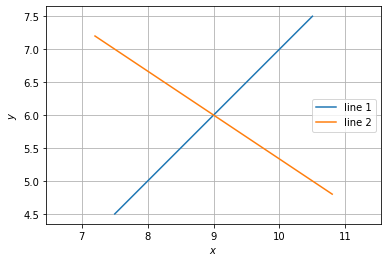
\includegraphics[width=\columnwidth]{solutions/quad/45/figure2.png}
\caption{Rhombus ABCD}
\label{quad/45/fig:Rhombus ABCD}
\end{figure}

\item Find the equation of set of points $\vec{P}$ such that
\begin{align}
PA^2+PB^2 =2k^2,
\end{align}
%
\begin{align}
\vec{A} = \myvec{3\\4 \\5},
\vec{B} = \myvec{-1\\3 \\-7},
\end{align}
%
respectively.
%
\item Find the coordinates of a point which divides the line segment joining the points \myvec{1\\-2\\3} and \myvec{3\\4\\-5} in the ratio $2:3$
\begin{enumerate}
\item internally, and
\item externally.
\end{enumerate}
%
\solution
We obtain the vertices of the rhombus as follows
\begin{align}
\vec{A} = \myvec{-3\\0},
\vec{B} = \myvec{0\\-3.5},
\vec{C} = \myvec{3\\0},
\vec{D} = \myvec{0\\3.5}
\end{align}
which are plotted in Fig. \ref{quad/45/fig:Rhombus ABCD}.
%
\begin{figure}[ht!]
\centering
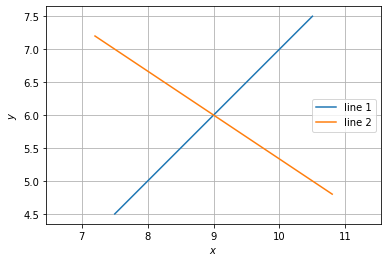
\includegraphics[width=\columnwidth]{solutions/quad/45/figure2.png}
\caption{Rhombus ABCD}
\label{quad/45/fig:Rhombus ABCD}
\end{figure}

%\solution Use \eqref{eq:line_section_form}.

\item Prove that the three points \myvec{-4\\6\\10}, \myvec{2\\4\\6} and \myvec{14\\0\\-2} are collinear.
%
\\
\solution 
%
We obtain the vertices of the rhombus as follows
\begin{align}
\vec{A} = \myvec{-3\\0},
\vec{B} = \myvec{0\\-3.5},
\vec{C} = \myvec{3\\0},
\vec{D} = \myvec{0\\3.5}
\end{align}
which are plotted in Fig. \ref{quad/45/fig:Rhombus ABCD}.
%
\begin{figure}[ht!]
\centering
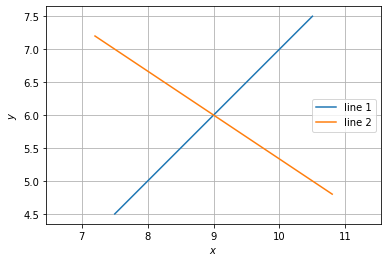
\includegraphics[width=\columnwidth]{solutions/quad/45/figure2.png}
\caption{Rhombus ABCD}
\label{quad/45/fig:Rhombus ABCD}
\end{figure}

%
\item Find the ratio in which the line segment joining the points \myvec{4\\8\\10} and \myvec{6\\10\\-8} is divided by the YZ-plane.
%
%\\
%\solution Use \eqref{eq:line_section_form}.  The YZ-plane has points \myvec{0\\y\\z}.
%
\item Find the equation of the set of points $\vec{P}$ such that its distances from the points
$
\vec{A}=\myvec{3\\4\\-5}, 
\vec{B}=\myvec{-2\\1\\4}
$
are equal. 
%
%\\
%\solution Use the approach in Problem \ref{prob:line_perp_bisect}.
\item If 
\begin{align}
\vec{P} = 3\vec{a}-2\vec{b}
\\
\vec{Q} = \vec{a}+\vec{b}
\end{align}
%
find $\vec{R}$, which divides $PQ$ in the ratio $2:1$
\begin{enumerate}
\item internally,
\item externally.
\end{enumerate}
%
\item Find a unit vector in the direction of \myvec{2\\-1\\-2}.
%
\item Find a unit vector in the direction of the line passing through \myvec{-2\\4\\-5} and $\myvec{1\\2\\3}$.
%
\item Find a unit vector in the direction of $\vec{a}+\vec{b}$, where 
%
\begin{align}
\vec{a} = \myvec{2\\2\\-5}, \vec{b} = \myvec{2\\1\\3}.
\end{align}
%
\item Find a unit vector in the direction of 
%
\begin{align}
\myvec{1\\1\\-2}.
\end{align}
%
\item Find a point on the $y$-axis which is equidistant from the points $\vec{A} = \myvec{6\\5}, \vec{B} = \myvec{-4\\3}$.

\item The line through the points \myvec{-2\\6} and \myvec{4\\8} is perpendicular to the line through the points \myvec{8\\12} and $\myvec{x\\24}$.  Find the value of $x$.

%\end{enumerate}
%

